\Needspace{24\baselineskip}
\section{Results}\label{sec:results}
The whole-game comparison measured score, level completion, game overs, actions, and token usage on the 25 public games. The controlled tests then examined the level-brief package under the decision rule set in advance. The final subsection reports on the runs that did not win and on earlier tests that found no detectable benefit.

\subsection{The layered runs scored 85.37\% RHAE and the baseline scored 46.20\%}\label{sec:result-score}
Across 25 public games, the layered harness scored 85.37\% RHAE and the baseline scored 46.20\% (Table~\ref{tab:main}). The difference, calculated from the unrounded scores, was 39.17 percentage points. The comparison included one recorded baseline run and one recorded layered run per game, including runs that halted before winning. The layered runs completed 166 of 183 levels and won 17 of 25 games. The baseline completed 125 levels and won seven games. The layered runs used 10,686 actions, compared with 16,560 for the baseline. For example, the layered harness won \texttt{dc22} in 619 actions and \texttt{re86} in 655, while the baseline used its full caps of 1,250 and 1,300 actions on those games and won neither. Both scorecards covered all 25 games \citep{scorecard2026baselinefinal,scorecard2026finalreplay,dai2026baselinefinalcard,dai2026finalmanifest}.

\begin{table}[htbp]
\centering\small
\begin{tabularx}{\linewidth}{@{}Yrrrr@{}}\toprule
Competition-mode replay & RHAE (\%) & Levels & Games won & Actions\\\midrule
\multicolumn{5}{@{}l}{\emph{The comparison: same model and same per-game action caps}}\\
\quad\textbf{Baseline} & \textbf{46.20} & \textbf{125/183} & \textbf{7/25} & \textbf{16,560}\\
\quad\textbf{Layered harness} & \textbf{85.37} & \textbf{166/183} & \textbf{17/25} & \textbf{10,686}\\\midrule
\multicolumn{5}{@{}l}{\color{black!60}\emph{For reference: the same baseline runs after their first 100 actions per game}}\\
\quad\color{black!60}Baseline, first 100 actions & \color{black!60}23.16 & \color{black!60}67/183 & \color{black!60}1/25 & \color{black!60}2,475\\\bottomrule
\end{tabularx}
\caption{The evaluation covered 25 public games, with one recorded run from each harness per game, including halted runs. The two rows in bold are the comparison this paper reports. Both include every recorded action from all 25 ended or halted runs, and the layered runs started from the first action under the extended baseline's cap table. The gray row is not a third condition: it shows the same baseline runs after their first 100 actions per game, before the continuations. ARC-service action replay confirmed all three scores. Resets count as actions. These self-run records do not imply independent leaderboard verification.}\label{tab:main}\label{tab:full-comparison}
\end{table}


Additional actions did not necessarily increase the score. On \texttt{wa30}, the layered harness completed seven of nine levels and used all 1,850 allowed actions. It scored 52.68\%, compared with the baseline's 41.44\%. The agent completed the seventh level at action 1,560. The remaining 290 actions completed no further level, so they used tokens and left the score unchanged.

\subsection{Completion improved in 15 of 25 games and declined in one}\label{sec:result-completion}
The layered harness completed more levels than the baseline in 15 games, the same number in nine, and fewer in one (Figure~\ref{fig:per-game-outcomes}a). It scored higher in 20 games and lower in one (Figure~\ref{fig:per-game-outcomes}b). In the other four games, both harnesses won with scores of 100\%. The only decline in either completion or score occurred on \texttt{s5i5}. The baseline won that game, while the layered run halted after completing six of eight levels. Table~\ref{tab:layered-games} reports each game's final outcome, including runs halted by timeouts.

\begin{figure}[htbp]
\centering
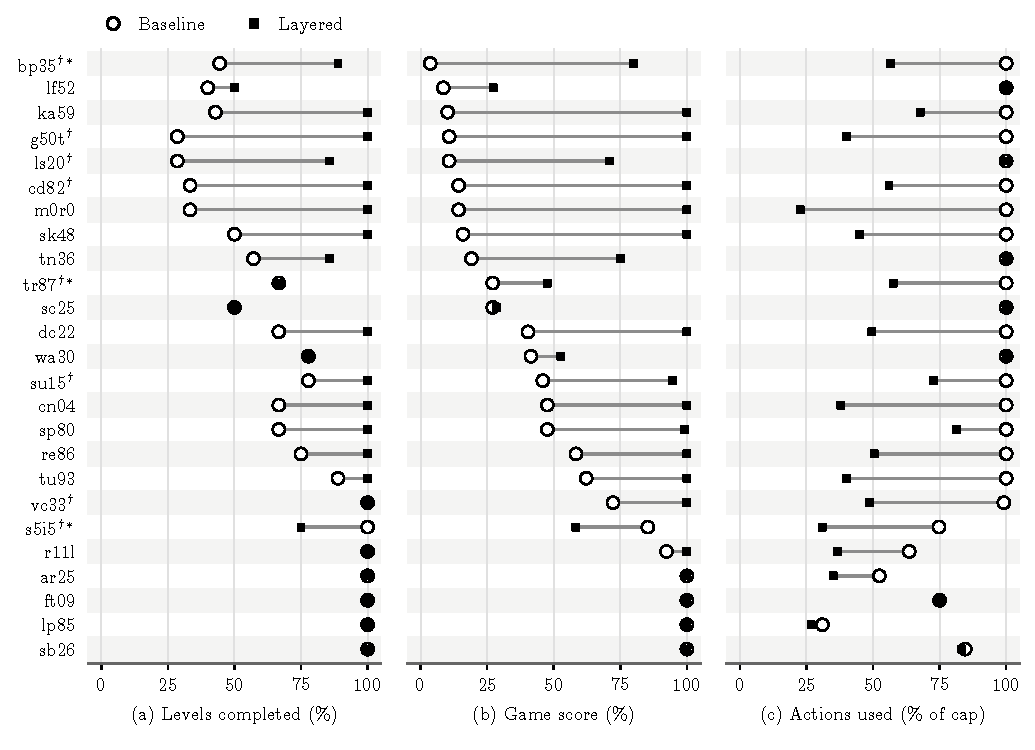
\includegraphics[width=\linewidth]{figures/per_game_outcomes.pdf}
\caption{\textbf{In most games the layered run completed more levels and scored higher while using fewer actions.} Each row compares one baseline run and one layered run on the same game. The rows run from the lowest baseline score to the highest. Open circles show the baseline results, filled squares show the layered results, and a line connects the two. The panels show (a) the percentage of levels completed, (b) the game score, and (c) the percentage of the game's action cap used. Both harnesses had the same cap for each game. A dagger marks games used or studied during development. An asterisk marks layered runs stopped by repeated timeouts; the figure reports their results at the point they stopped. The layered harness completed more levels in 15 games, the same number in nine, and fewer in one (\texttt{s5i5}). It scored higher in 20 games and used fewer actions in 19. The connecting lines show differences between two recorded runs; they do not show statistical uncertainty. Table~\ref{tab:layered-games} gives the exact values.}\label{fig:per-game-outcomes}
\end{figure}

Most of the additional completed levels came from games on which the baseline scored below 40\%. These 11 games formed the first of the three batches of layered runs (Section~\ref{sec:design}). The layered harness completed 66 levels on them, compared with 34 for the baseline, and raised the mean score from 14.69\% to 75.39\%. These 11 games accounted for 32 of the 41 additional levels. On the six games in that set outside the eight-game development group, completion increased from 20 to 35 levels and mean score from 15.86\% to 71.81\%. On the second batch of 11 games, the layered harness completed 79 levels and the baseline completed 74. On the final batch of three games, the layered harness completed 21 levels and the baseline completed 17 \citep{dai2026layered}.

The layered harness had a higher mean score than the baseline in each development-exposure group (Table~\ref{tab:layer-exposure}). On the 17 games outside the eight-game development group, mean score increased from 52.06\% to 87.22\%. On the eight games within that group, it increased from 33.74\% to 81.44\%. Neither group is a held-out test set, because baseline failures on all 25 games informed development (Section~\ref{sec:design}).

\begin{table}[H]
\centering\small
\begin{tabularx}{\linewidth}{@{}Yrrrr@{}}\toprule
Development exposure & Games & \shortstack{Mean score\\baseline / layered} & \shortstack{Levels\\baseline / layered} & \shortstack{Action totals\\baseline / layered}\\\midrule
Other games & 17 & 52.06 / 87.22 & 89 / 113 & 12,178 / 8,048\\
Used or studied & 8 & 33.74 / 81.44 & 36 / 53 & 4,382 / 2,638\\\bottomrule
\end{tabularx}
\caption{The table reports results by development exposure on 25 games, with one run per condition per game, including halted runs. Each pair reports the baseline value followed by the layered value. The eight-game group contains games used to design or tune a layer, or studied during development. Work on \texttt{g50t} consisted of ledger tests and replay study. The other 17 games include \texttt{wa30}. Baseline failures on all 25 games informed development, so neither group is a held-out test set.}\label{tab:layer-exposure}
\end{table}

\subsection{The layered runs had fewer game overs}\label{sec:result-game-overs}
The introduction's example was a repeated game over, so I counted game overs in both sets of runs. The baseline had 127 in 16,560 actions, and the layered runs had 36 in 10,686 actions, or 0.77 and 0.34 per 100 actions. On \texttt{bp35}, the game in that example, the baseline had 22 game overs in 700 actions and the layered run had 5 in 397. These counts include every game over, so they do not show how many repeated an earlier mistake. The baseline count is the number of level resets in its recorded actions: the controller sent one after each game over, and no baseline run ended on a game over \citep{dai2026baselineactions,dai2026layered}.

\subsection{Actions on unfinished levels decreased from 7,940 to 2,170, and reported tokens decreased by 11.0\%}\label{sec:result-resources}
The layered runs used 35.5\% fewer actions overall, 10,686 compared with 16,560. They used fewer actions in 19 games and the same number in six (Figure~\ref{fig:per-game-outcomes}c).

Nearly all of this reduction came from actions used on levels that were unfinished when the runs ended. The baseline used 7,940 actions on its unfinished levels, compared with 2,170 for the layered harness on its unfinished levels. That is a decrease of 5,770 actions, out of an overall decrease of 5,874. The totals for actions used on completed levels were similar, 8,620 for the baseline and 8,516 for the layered harness. Those totals covered different sets of completed levels, with 125 for the baseline and 166 for the layered harness. Relative to the human-baseline action count, the layered harness completed 151 levels at or below that count, compared with 86 for the baseline (Figure~\ref{fig:level-action-ratio}).

\begin{figure}[htbp]
\centering
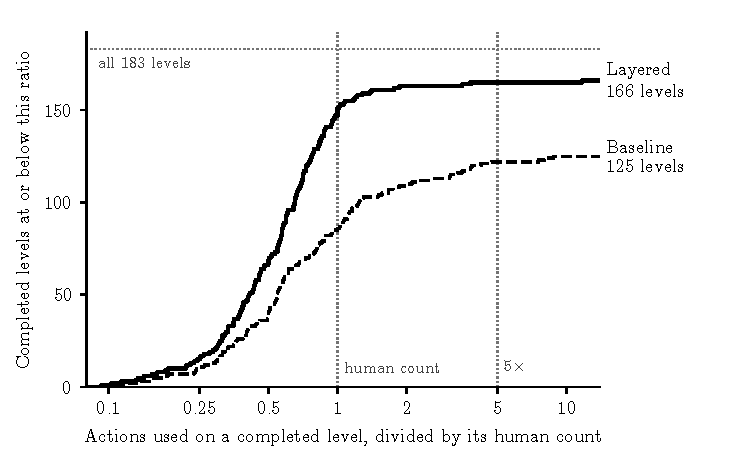
\includegraphics[width=0.74\linewidth]{figures/level_action_ratio.pdf}
\caption{\textbf{Both harnesses solved most of their completed levels within the human action count, and few levels took more than five times that count.} The horizontal axis shows the actions used to complete a level as a multiple of that level's human baseline: 1 means the same number of actions, and 5 means five times as many. The axis uses a logarithmic scale. At each point, a curve shows how many levels a harness completed using no more than that multiple. The solid curve shows the layered runs (166 completed levels), and the dashed curve shows the baseline (125). The vertical dotted lines mark 1 and 5; five times the human count is the official leaderboard's action budget for each level \citep{arc2026technical}. The horizontal dotted line shows the total of 183 levels. The layered harness completed 151 levels within the human action count, compared with 86 for the baseline. One completed level in the layered runs and three in the baseline took more than five times the human count. The curves exclude unfinished levels.}\label{fig:level-action-ratio}
\end{figure}

The overall action totals cover both completed and unfinished games, including runs stopped by timeouts. The three halted runs left 943 actions unused under their caps. On the other 22 games, the layered runs used 34.1\% fewer actions than the baseline, 9,829 compared with 14,924. If the three halted runs had used every remaining action, the overall reduction would have been 29.8\% rather than 35.5\%.

On the six games that both harnesses won, the baseline used 1,324 actions and the layered harness used 881, a reduction of 33.5\%. This subset does not represent performance across all 25 games. It excludes \texttt{s5i5}, which the baseline won and the layered run did not finish before it halted.

\begin{table}[H]
\centering\small
\begin{tabularx}{\linewidth}{@{}Yrrr@{}}\toprule
Reported measure, 25 games & Baseline & Layered & Reduction\\\midrule
Environment actions & 16,560 & 10,686 & 35.5\%\\
\quad on levels left unfinished & 7,940 & 2,170 & 72.7\%\\
\quad on completed levels & 8,620 & 8,516 & 1.2\%\\
Model replies with reported token counts & 16,433 & 11,111 & 32.4\%\\
Input tokens (millions) & 219.307 & 201.030 & 8.3\%\\
Output tokens (millions) & 37.194 & 27.316 & 26.6\%\\
Input plus output (millions) & 256.501 & 228.346 & 11.0\%\\\bottomrule
\end{tabularx}
\caption{The table reports usage for each condition across 25 games, including halted runs and \texttt{wa30}. Reduction is relative to the baseline. The two indented rows split the actions by whether the agent completed the level; the completed levels differ between the harnesses (125 and 166). Reply and token totals include rejected replies retained in the final records; Appendix~\ref{app:continuation} describes the exclusions. Output already includes thinking tokens. Calls stopped by timeouts reported no usage, so the totals for both harnesses exclude them. The layered runs had 97 such calls (Section~\ref{sec:continuation-design}). The totals do not measure total compute consumed or billing savings.}\label{tab:tokens}
\end{table}

Reported token usage decreased by 11.0\%, compared with the 35.5\% reduction in actions (Table~\ref{tab:tokens}). The layered harness used longer requests, and reported input tokens per environment action were 42.1\% higher with the layers. I calculated this average by dividing total reported input tokens by total executed environment actions. On \texttt{wa30}, both the baseline and layered harnesses used 1,850 actions and completed seven levels, but reported tokens increased from 28.408 million to 39.208 million. Including this game reduced the token saving from the earlier 24-game estimate of 17.1\% to 11.0\% across all 25 games \citep{dai2026tokens}.

Two cautions apply to these totals. Calls stopped by timeouts reported no usage, so the totals do not establish a reduction in total compute consumed. The totals do include the extra model calls that the layered harness needed to correct rejected replies: 4.1\% of its replies tried to add a rule to a full list without naming one to replace, and the harness returned them for correction (Section~\ref{sec:continuation-design}).

\subsection{Applying the leaderboard's per-level budget changed each score by less than 0.3 points}\label{sec:result-budget}
The action budget in this study differed from the official leaderboard's. The leaderboard stops an agent at five times the human-baseline action count on each level, whereas this study limited each game's total actions \citep{arc2026technical}. To see how much this difference mattered, I applied the leaderboard's budget to the saved action sequences. For each game, I stopped the saved action sequence when the agent exhausted a level's budget before completing that level, and I discarded all later actions in that game. Applying this cutoff without new model decisions gave scores of 45.92\% for the baseline and 85.13\% for the layered harness, a difference of 39.20 percentage points when calculated from the unrounded scores.

This cutoff removed one completed layered level, the seventh level of \texttt{wa30}, which took 921 actions against a human count of 79. It removed four completed baseline levels. Three exceeded the budget (Figure~\ref{fig:level-action-ratio}) and one followed a level that exceeded the budget in the same game. The calculation could only remove actions from the saved runs. It cannot show what either agent would have done if a different budget had allowed play beyond the study's whole-game action cap.

\subsection{The level-brief package met its benefit criterion in one of two tests}\label{sec:result-brief}
The configuration with the package completed more levels in both test sets, but only the second set met the benefit criterion set in advance (Table~\ref{tab:brief}, Figure~\ref{fig:brief-tests}). In the first set, the package added seven completed levels overall but completed one fewer level on \texttt{wa30}. It therefore failed the requirement to match or exceed completion in every game and received the rule's label \emph{no detectable difference}. In the second set, it added nine completed levels, improved completion in five games, and reduced it in none, meeting the criterion for \emph{helps} \citep{dai2026brieftests}.

\begin{table}[H]
\centering\small
\begin{tabularx}{\linewidth}{@{}YrrrY@{}}\toprule
Test set & Games & \shortstack{Levels\\without / with} & \shortstack{Games\\ahead / behind} & Verdict under the rule\\\midrule
First set & 7 & 10 / 17 & 4 / 1 & No detectable difference\\
Second set & 9 & 29 / 38 & 5 / 0 & Helps\\\bottomrule
\end{tabularx}
\caption{The controlled tests of the level-brief package used two runs per configuration per game and up to 100 new actions per run, stopping early on a win. Runs began from specified restored positions, except \texttt{tn36}, which started at the first action. The configuration without the package retained the other memory layers and object ledger. Level counts sum the two runs for each configuration and include only levels completed during the new actions. Ahead and behind count games where this sum was higher or lower with the package enabled. Verdicts follow the rule set in advance, applied separately to each set (Section~\ref{sec:brief-design}). They are not statistical significance tests.}\label{tab:brief}
\end{table}

\begin{figure}[htbp]
\centering
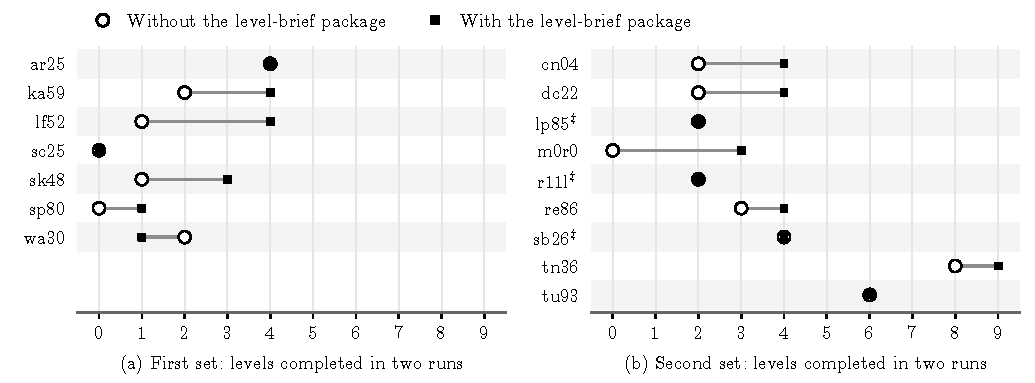
\includegraphics[width=\linewidth]{figures/brief_tests.pdf}
\caption{\textbf{The level-brief package completed more levels in both test sets and completed fewer in one game of the first.} Each row is a game. The horizontal position is the number of levels completed in two runs of up to 100 new actions each. Open circles are the runs without the package, which kept the other memory layers and the object ledger. Filled squares are the runs with it. (a) In the first set, the package was ahead in four games, behind in one (\texttt{wa30}), and level in two, with 17 levels against 10. (b) In the second set, the package was ahead in five games, behind in none, and level in four, with 38 levels against 29. A double dagger marks a game that every run won, so the counts could not differ. Each point sums two runs, and the figure draws no interval.}\label{fig:brief-tests}
\end{figure}


In the second set, every run on \texttt{lp85}, \texttt{r11l}, and \texttt{sb26} won in both tested harness configurations, so the number of completed levels could not distinguish the configurations on those games. These tests do not establish a general benefit or isolate the contributions of persistent rules, completion feedback, the brief, or the flags for newly observed appearance groups. They also did not test the removal of individual layers from whole-game runs.

\subsection{Eight layered runs did not win, and earlier tests gave null or negative results}\label{sec:result-failures}
Eight layered runs did not win. Repeated calls exceeding the time limit halted three of them: after four of six levels on \texttt{tr87}, eight of nine on \texttt{bp35}, and six of eight on \texttt{s5i5}. I retained each run's counts at the point it stopped. The baseline won \texttt{s5i5}, making it the only game in which the layered harness completed fewer levels. The other five runs used their whole action cap: \texttt{wa30} (seven of nine levels), \texttt{ls20} and \texttt{tn36} (six of seven each), \texttt{lf52} (five of ten), and \texttt{sc25} (three of six). Of these five, \texttt{sc25} and \texttt{wa30} ended with the same number of completed levels as the baseline, and \texttt{lf52} with one more.

Four earlier tests during development gave null or negative results. First, stating the scoring rule in the prompt showed no detectable benefit. At 50 saved turns where the baseline had taken an action with no effect, 31 replies chose that action again with the rule in the prompt and 28 without it. Second, I stopped a study of whether the model should reset a level. In its test at ten saved positions, none of 100 replies chose a reset, whether or not the prompt asked the model to consider one. Third, lessons after game overs showed no detectable effect when tested over a whole level. All four runs of \texttt{bp35} level 2, two with the lessons and two without, completed the level. Fourth, an agent with the level brief did not complete \texttt{tr87} level 2 during development \citep{dai2026negatives}. None of these tests showed that the feature it tested helps on its own.
